\section{System Architecture}
\label{sec:architecture}

\begin{designbox}
Give every component one home in a three-plane model so that decision authority,
work execution, and evidence recording are physically separated and independently
auditable. Judgment is confined to the control and execution planes; the evidence
plane records the run but never decides it.
\end{designbox}

Argus is organized as three cooperating planes. The \textbf{control plane} holds
the roles and scheduler that decide \emph{what to run and whether it is done}.
The \textbf{execution plane} runs \emph{one mission at a time} against real
tools, providers, and budgets. The \textbf{evidence plane} records the run on an
append-only tape with usage accounting, credential redaction, and provenance
digests. Figure~\ref{fig:planes} shows the planes and their interfaces;
Figure~\ref{fig:architecture} is the accepted system schematic. The end-to-end
control path is a single spine:
\code{CLI} $\rightarrow$ \code{Manager.divide} (vertical selection)
$\rightarrow$ runtime wiring $\rightarrow$ \code{LifeSupervisor} (mission
scheduler) $\rightarrow$ \code{SkillLoop} $\rightarrow$ \code{SupervisedEngineer}
$\leftrightarrow$ Reviewer-until-done, resting on the core services, the single
anti-stall mechanism, the pluggable verticals, and the provider
backend.\footnote{Spine and module map: \srcpath{docs/ARCHITECTURE.md}. Plane
assignment cross-referenced in Appendix~\ref{app:evidencemap}.}

\begin{figure}[ht]
\centering
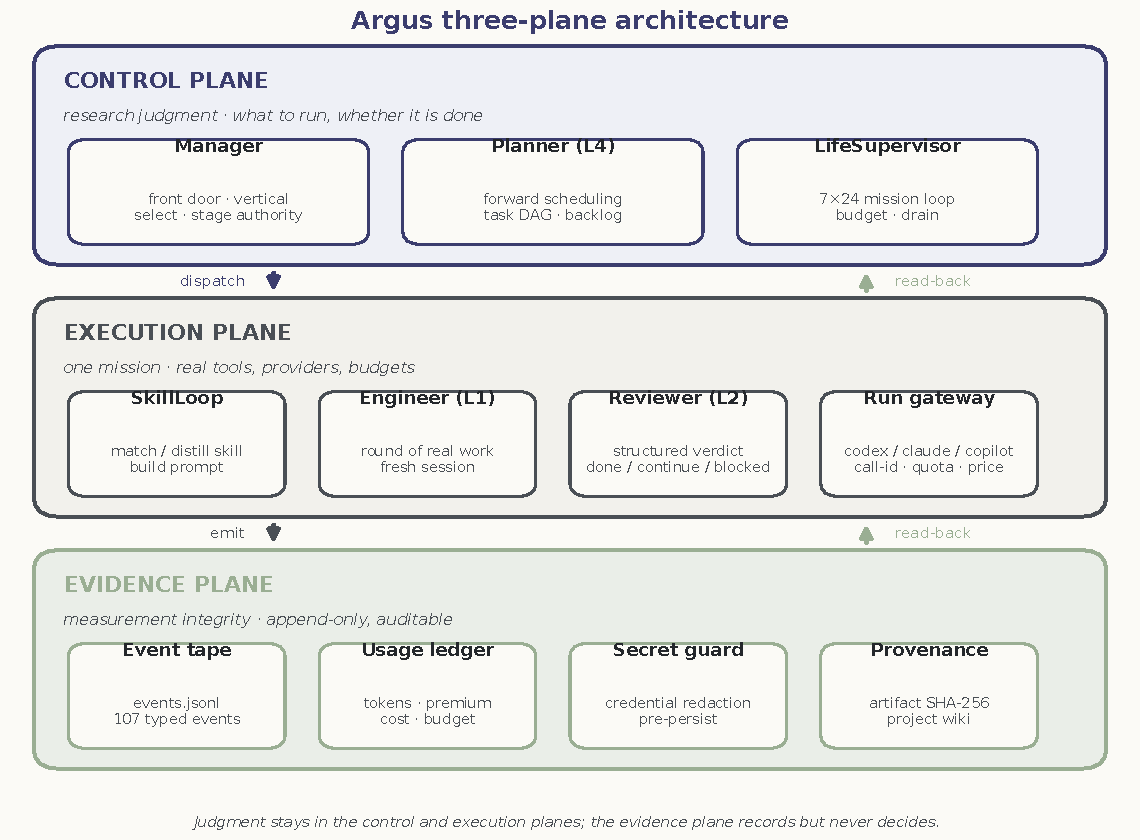
\includegraphics[width=\textwidth]{figures/system_planes.pdf}
\caption{The three-plane architecture. Control-plane roles dispatch work into the
execution plane, which emits typed events into the evidence plane; the evidence
plane is read back by both other planes but holds no decision authority. Drawn
deterministically from the module map (Appendix~\ref{app:evidencemap}).}
\label{fig:planes}
\end{figure}

\subsection{Control plane: decision authority}

The control plane is where scientific and scheduling authority live. The
\textbf{Manager} (\srcpath{manager/\_core.py}, \srcpath{manager/front\_door.py},
\srcpath{manager/dispatch.py}) is the single operator entry point: one grounded
model call routes free text to chat or task, selects the task shape
(\emph{vertical}) or authors a new data domain, and commits that choice durably.
It is also the \emph{sole} authority for pipeline-stage transitions --- it owns
the \code{current\_stage} field, and the other roles may only advise a change.
The \textbf{Planner} (\srcpath{planner/planner.py}) is the forward scheduler: it
proposes the next batch of work as a task DAG when the backlog empties. The
\textbf{LifeSupervisor} (\srcpath{life/supervisor/\_core.py}) is the 7$\times$24
outer loop that claims backlog items, runs missions, accounts cost, and plans
next. These components decide; they do not themselves touch a provider.

\subsection{Execution plane: one mission at a time}

The execution plane runs a single mission. \code{SkillLoop} (\srcpath{loop.py})
is the per-mission glue: it matches or distills a reusable skill, builds the
Engineer prompt, and drives the Engineer$\leftrightarrow$Reviewer round loop. The
\textbf{Engineer} (\srcpath{engineer/runner.py}) performs one round of real work
--- literature search, code, experiments, or writing --- and the \textbf{Reviewer}
(\srcpath{reviewer/\_core.py}) returns a structured verdict. Every provider call,
regardless of role, is issued through a single application-level gateway
(\srcpath{core/run\_gateway.py}), which assigns a \code{call\_id}, propagates the
resume-thread identity, and stamps timing --- one interception point for tracing,
metrics, and policy. The concrete backends (Codex, Claude Code, GitHub Copilot
CLI) sit behind an adapter (\srcpath{adapters/agent\_cli\_backend.py}); a
deterministic in-memory backend (\srcpath{adapters/memory\_backend.py}) drives
tests.

\subsection{Evidence plane: measurement integrity}

The evidence plane records the run and enforces the run's integrity invariants
(Section~\ref{sec:evidence}). Its spine is a per-project append-only
event tape, \code{events.jsonl} (\srcpath{core/paths.py}), carrying the 112 typed
event types. Alongside it sit the usage ledger (\srcpath{core/usage.py}), the
credential-redaction pass applied before persistence
(\srcpath{core/secret\_guard.py}), the provenance and artifact-corroboration
records (\srcpath{skills/provenance.py}, \srcpath{webapi/artifacts.py}), and the
project wiki of immutable, evidence-cited pages (\srcpath{argus\_skill/wiki/}).
Nothing in this plane makes a scientific decision; it exists so that a decision
made elsewhere can be checked.

\subsection{Module map}

Table~\ref{tab:modmap} maps each area of the live tree to its plane and files.
The map is authoritative in \srcpath{docs/ARCHITECTURE.md} and is kept in sync
with the code.

\begin{table}[t]
\centering
\small
\begin{tabularx}{\linewidth}{@{}p{2.4cm} p{2.0cm} X@{}}
\toprule
\textbf{Area} & \textbf{Plane} & \textbf{Primary file(s)} \\
\midrule
Entry / CLI        & control  & \code{apps/cli/\_parser.py}, \code{apps/cli/\_core.py}, \code{\_\_main\_\_.py} \\
Manager            & control  & \code{manager/\_core.py}, \code{manager/front\_door.py}, \code{manager/dispatch.py} \\
Planner            & control  & \code{planner/planner.py}, \code{planner/planner\_schema.json} \\
Mission scheduler  & control  & \code{life/supervisor/\_core.py} \\
Daemon             & control  & \code{daemon/life\_worker.py}, \code{daemon/handoff.py} \\
Skill loop         & execution& \code{loop.py} \\
Engineer           & execution& \code{engineer/runner.py}, \code{engineer/checkpoint.py} \\
Reviewer           & execution& \code{reviewer/\_core.py}, \code{reviewer/reviewer\_schema.json} \\
Provider gateway   & execution& \code{core/run\_gateway.py}, \code{adapters/agent\_cli\_backend.py} \\
Anti-stall (meta)  & execution& \code{regime\_jump/} (saturation, flow, ledger, meta-prompter) \\
Verticals          & execution& \code{verticals/} --- nanochat, nanogpt\_speedrun, kernelbench, research, \ldots \\
Core services      & evidence & \code{core/paths.py}, \code{core/usage.py}, \code{core/pricing.py}, \code{core/models.py} \\
Integrity          & evidence & \code{core/secret\_guard.py}, \code{skills/provenance.py} \\
Event catalog      & evidence & \code{core/event\_catalog.py}, \code{core/event\_payload\_schemas.json} \\
Cockpit            & (all)    & \code{webapi/server.py}, \code{frontend/tui/}, \code{frontend/web/} \\
\bottomrule
\end{tabularx}
\caption{Module map, by plane. Areas marked ``(all)'' observe across planes but
hold no decision authority. Full table: \srcpath{docs/ARCHITECTURE.md}.}
\label{tab:modmap}
\end{table}

\begin{figure}[ht]
\centering
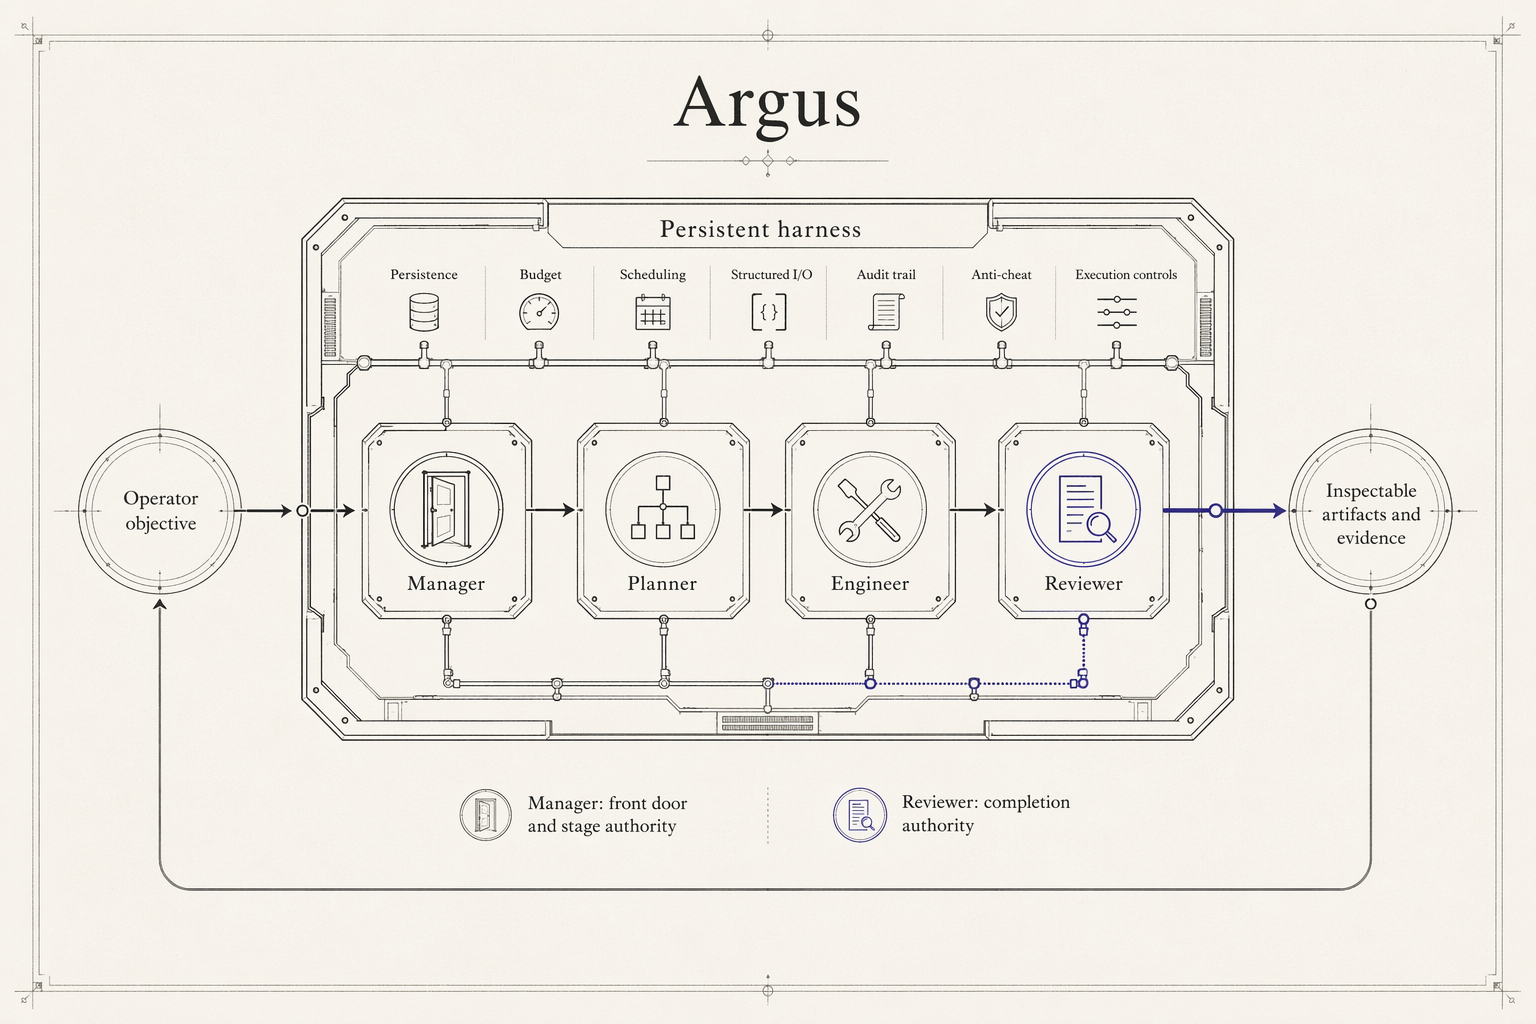
\includegraphics[width=0.6\textwidth]{figures/argus_architecture.png}
\caption{System schematic (not a measured performance plot): an operator
objective enters the persistent runtime; the Manager, Planner, Engineer, and
Reviewer sit inside it as the four roles that carry every research judgment; and
inspectable artifacts and evidence exit back to the operator.}
\label{fig:architecture}
\end{figure}

\subsection{What is deliberately not in the spine}

Two things are kept off the default path. The research-paper pipeline (the
\code{research} vertical and its paper machinery) is lazy-loaded only when a
project's vertical is \code{research}; it is not part of the metric-reproduction
product. And a \textbf{Curator} role (skill-pool maintenance, team-leaderboard
distillation) runs only in team mode. Both are described where they are used
(Sections~\ref{sec:state}, \ref{sec:portfolio}) rather than as spine components.
